Ideę rozbijania rozkładu na dwuwymiarowe bloki da się rozszerzyć na $d$-wymiarów. Podobnie jednak jak w przykładzie 3-wymiarowym z sekcji \ref{subsub:przyklad_3_wymiary}, nie mamy jedyności tej reprezentacji - istnieje wiele różnych dróg do osiągnięcia tego samego celu. 

\begin{thm}[$d$-wymiarowa PCC]
	Niech $f_{1,2,\dots,d}$ będzie gęstością łączną $d$-wymiarowego rozkładu. Możemy ją wyrazić poprzez:
	
	\begin{equation}
		f_{1,\dots, d}(x_1, \dots, x_d) = \bigg[ \prod_{j=1}^{d-1} \prod_{i=1}^{d-j} c_{i, (i+j); (i+1)\dots(i+j-1)} \bigg] \cdot \bigg[ \prod_{k=1}^{d}f_k(x_k)\bigg].
		\label{eq:recursive_pcc}
	\end{equation}
\end{thm}
\begin{proof}
	Zacznijmy od rozważenia rozkładu łącznego i jego ogólnej rekursywnej dekompozycji:
\begin{equation}
	\begin{split}
		f_{1, \dots, d}(x_1, \dots, x_d) &= f_{d|1 , \dots, d-1}(x_d|x_1, \dots, x_{d-1})f_{1,\dots,d-1}(x_1, \dots, x_{d-1})\\
		&=\dots= \bigg[\prod_{t=2}^{d}f_{t|1,\dots,t-1}(x_t|x_1, \dots, x_{t-1})\bigg]\cdot f_1(x_1)
	\end{split}
	\label{eq:d-dimensional_decomp}
\end{equation}

Teraz użyjemy lematu \ref{lem:copula_representation_of_conditional_density} do rozkładu warunkowego $(X_1, X_t) | (X_2, \dots, X_{t-1})$ żeby wyrazić $f_{t|1,\dots,t-1}(x_t|x_1,\dots,x_{t-1})$.
	\begin{equation}
	\begin{split}
	f_{t|1,\dots,t-1}(x_t|x_1,\dots,x_{t-1})&= c_{1,t|2,\dots,t-1}\cdot f_{t|2,\dots,t-1}(x_t|x_2,\dots,x_{t-1})  \\
	& = \bigg[ \prod_{s=1}^{t-2} c_{s,t;s+1,\dots,t-1} \bigg] c_{(t-1), t} f_t(x_t).	
	\end{split}
	\end{equation}

Aplikując \ref{eq:recursive_pcc} do równania \ref{eq:d-dimensional_decomp}, oraz oznaczając $s=i, t=i+j$ możemy zapisać:

\begin{equation*}
	\begin{split}
		f_{1, \dots, d}(x_1, \dots, x_d) &= \bigg[\prod_{t=2}^{d}\prod_{s=1}^{t-2} c_{s,t;s+1,\dots,t-1}\bigg] \cdot \bigg[ \prod_{t=2}^{d}c_{(t-1), t} \bigg] \cdot \bigg[ \prod_{k=1}^{d}f_{k}(x_k) \bigg] = \\
		& = \bigg[\prod_{j=1}^{d-1}\prod_{i=1}^{d-j}c_{i,(i+j);(i+1)\dots(i+j-1)}\ \bigg] \cdot \bigg[\prod_{k=1}^{d}f_k(x_k)\bigg].
	\end{split}
\end{equation*}
\end{proof}

Jak widać z równania \ref{eq:d-dimensional_decomp}, dekompozycje te potrafią być zawiłe i mało interpretowalne. Do tego dochodzi fakt, że podobnie jak w przykładzie 3-wymiarowym, nie jest to jedyna postać dekompozycji. Dlatego wprowadzimy teraz fragmenty teorii grafów, która pozwoli nam lepiej komunikować i zrozumieć strukturę PCC.

\begin{df}[Graf, wierzchołek, krawędź, stopień]
	Grafem nazwiemy parę zbiorów $G= (N, E)$, takich że $E \subseteq \{ \{x,y \}: x,y \in N \}$.
	\begin{itemize}
		\item Elementy $E$ nazywać będziemy krawędziami grafu $G$, a elementy $N$ wierzchołkami
		\item Liczbę sąsiadów wierzchołka $v\in N$ będziemy nazywać jego stopniem i oznaczać $d(v)$
	\end{itemize}
\end{df}

\begin{df}[Ścieżka, cykl, graf spójny, graf acykliczny]
	Ścieżka to rodzaj grafu $P = (N, E)$ o wierzchołkach $N = \{ v_0, v_1, \dots, v_k\}$ i krawędziach \\ $E = \{ \{v_0, v_1 \}, \{v_1, v_2 \}, \{v_2, v_3 \}, \dots, \{v_{k-1}, v_k \} \}$.\\
	Cyklem nazywamy ścieżkę gdzie $v_0=v_k$.\\
	Jeżeli dla każdej pary wierzchołków istnieje łącząca je ścieżka, to graf nazwiemy spójnym. Jeżeli graf nie zawiera w sobie cykli, to nazwiemy go acyklicznym. 
\end{df}

\begin{figure}[h]
	\centering
	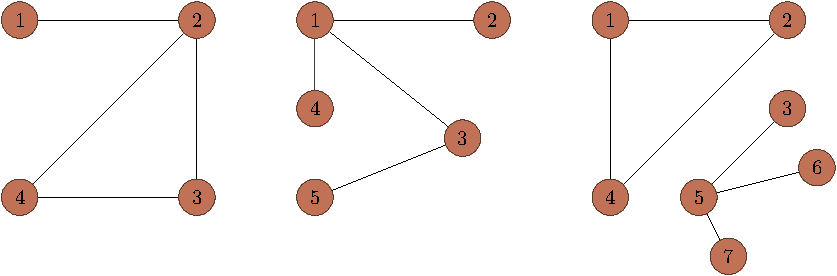
\includegraphics[width=\linewidth]{03_example_graph}
	
	\caption{Przykłady grafów: cykliczny spójny (po lewej), acykliczny spójny (na środku), cykliczny niespójny (po prawej)\label{fig:example_graph}}
\end{figure}

Przykładowe grafy przedstawione sa na rysunku \ref{fig:example_graph}. Nas interesować będą jednak szczególne rodzaje grafów, nazywane drzewami.
\begin{df}[Charakteryzacja drzewa]
	Poniższe stwierdzenia są równoważne dla grafu $T = (N, E)$:
	\begin{enumerate}
		\item $T$ jest drzewem
		\item Dowolne dwa węzły grafu $T$ są połączone unikalną ścieżką w $T$.
		\item $T$ jest grafem spójnym, ale $T-e$ jest niespójnym dla dowolnej krawędzi $e\in E$
		\item $T$ jest grafem acyklicznym, ale $T +\{x,y\}$ będzie zawierać cykl dla dowolnych dwóch niesąsiadujących wierzchołków $x, y \in N$.
	\end{enumerate}
\end{df}

Jedynym drzewem widocznym na rysunku \ref{fig:example_graph} jest graf na środkowym panelu. Drzewa są istotne w teorii wielowymiarowych kopuł, ponieważ stanowią podstawowy element budujący \emph{regular vines}, czyli zbiory grafów które posłużą nam do przedstawiania struktury PCC.

\begin{df}[Regular vine]
	Zbiór drzew $\Nu = (T_1,\dots, T_{d-1})$ nazywamy \emph{regular vine}, lub \emph{R-vine} jeżeli:
	
	\begin{enumerate}
		\item Każde drzewo $T_j=(N_j, E_j)$ jest spójne
		\item $T_1$ jest drzewem o zbiorze wierzchołków $N_1$ i zbiorze krawędzi $E_1$
		\item Dla $j\geqslant2$, $T_j$ jest drzewem o zbiorze wierzchołków $N_j = E_{j-1}$ i zbiorze krawędzi $E_{j-1}$
		\item Dla $j = 2, \dots, d- 1$ oraz $\{a, b\} \in E_j$ mamy $ \vert a \cap b \vert = 1$. 
	\end{enumerate}
\end{df}

Na wykresie \ref{fig:r_vine} pokazujemy przykładową strukture R-vine. Opisu krawędzi i wierzchołków dokonujemy zgodnie z wprowadzanym poniżej pojęciem warunkowego i warunkowanego zbioru.

\begin{df}[Zbiór warunkowy, zbiór warunkowany]
	Dla dowolnej krawędzi $e\in E_i$ zdefiniujmy zbiór:
	$$ A_e\coloneqq \{j\in N_1\vert \exists e_1 \in E_1, \dots, e_{i-1}\in E_{i-1}: j\in e_1\in \dots \in e_{i-1}\in e\}.$$
	Zbiorem warunkującym $D_e$ krawędzi $e=\{a, b\}$ nazywamy:
	
	$$ D_e \coloneqq A_a \cup A_b,$$
	
	zbiorami warunkowanymi $C_{e, a}$ i $C_{e, b}$ nazywamy natomiast:
	
	$$ C_{e, a} \coloneqq A_a\\ D_e$$
	$$ C_{e, b} \coloneqq A_b\\ D_e.$$
	
	Skrótowo, będziemy opisywać krawędź $e = (C_{e, a}, C_{e, b}; D_e)$ jako $e = (e_a, e_b; D_e)$.
\end{df}


\begin{figure}[h]
	\centering
	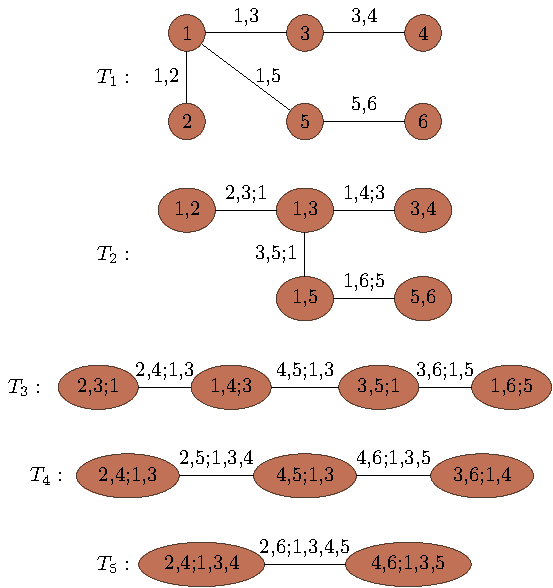
\includegraphics[width=0.7\linewidth]{03_R_vine}
	
	\caption{Przykładowa 6-wymiarowa struktura R-vine. \label{fig:r_vine}}
\end{figure}

Definicja struktury R-vine nie narzuca szczególnej postaci drzew. Jeżeli zaczniemy stawiać pewne warunki na ich strukturę, to trafimy w szczególności w dwie podklasy: D-vine i C-vine (rysunek \ref{fig:d_vine_c_vine}). D-vine zachodzi gdy każdy wierzchołek ma stopień co najwyżej równy dwa - powoduje to że drzewa wyglądają jak łańcuchy i nie mają odgałęzień. C-vine natomiast pojawia się w przypadku gdy każde drzewo ma pewien \emph{root node}, który jest połączony z każdym innym wierzchołkiem.
\begin{df}[D-vine, C-vine]
	Niech $\Nu$ będzie strukturą R-vine.
	\begin{enumerate}
		\item Jeżeli dla każdego wierzchołka $n\in N_i$ zachodzi warunek $\vert \{e\in E_i\vert n\in e\}\vert \leqslant 2$, to należy ona do podklasy \emph{D-vine} (drawable vine).
		\item Jeżeli dla każdego drzewa $T_i$ istnieje wierzchołek $n\in N_i$ taki, że $\vert \{e\in E_i\vert n\in e\}\vert = d-i$, to należy ona do podklasy \emph{C-vine} (canonical vine).
	\end{enumerate}
\end{df}


\begin{figure}[h]
	\centering
	\begin{minipage}{0.35\linewidth}
	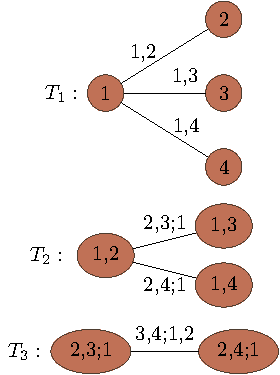
\includegraphics[width=\linewidth]{03_C_vine}
	\end{minipage}	
	\begin{minipage}{0.45\linewidth}
	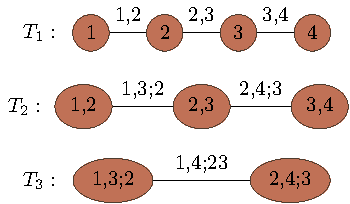
\includegraphics[width=\linewidth]{03_D_vine}
	\end{minipage}	

	\caption{Przykładowa 4-wymiarowa struktura C-vine (lewy panel) i D-vine (prawy panel). \label{fig:d_vine_c_vine}}
\end{figure}

Struktury R-vine są przydatne do wyjaśniania struktury zależności wielowymiarowych rozkładów, ponieważ jak pokazali \cite{BedfordCooke2002}, istnieje połączenie między PCC a pewnym R-vine.

\begin{df}[Rozkłady R-vine]
	Mówimy, że rozkład $F$ dla $d$-wymiarowego wektora losowego $(X_1, \dots, X_d)$ jest \emph{rozkładem R-vine}, jeśli możemy podać trójkę $(\mathcal{F}, \Nu, \mathcal{B})$ o własnościach:
	\begin{itemize}
		\item $\mathcal{F} =(F_1, \dots, F_d)$ jest wektorem ciągłych, odwracalnych dystrybuant rozkładów brzegowych $(X_1, \dots, X_d)$
		\item $\Nu$ jest $d$-wymiarową strukturą R-vine 
		\item Zbiór $\mathcal{B} = \{C_e\vert e \in E_i; i=1,\dots,d-1\}$, gdzie $C_e$ jest radialnie symetryczną dwuwymiarową kopułą posiadającą gęstość.
		\item Dla każdego $e\in E_i, i=1, \dots, d-1, e=\{a,b\}$, $C_e$ jest kopułą związaną z rozkładem warunkowym $X_{C_{e, a}}, X_{C_{e, b}}$ pod warunkiem $X_{D_e} = x_{D_e}$.
	\end{itemize}
	\label{def:r_vine_distribution}
\end{df}

W swojej pracy, Bedford i Cooke pokazują w szczególności, że dowolną trójkę $(\mathcal{F}, \Nu, \mathcal{B})$ o własnościach z definicji \ref{def:r_vine_distribution} można związać z pewnym $d$-wymiarowym rozkładem $F$.

\begin{thm}[Istnienie rozkładu R-vine]
	Niech $(\mathcal{F}, \Nu, \mathcal{B})$ spełnia warunki z definicji \ref{def:r_vine_distribution}. Wtedy istnieje dokładnie jeden $d$-wymiarowy rozkład $F$ o gęstości:
	
	\begin{equation*}
		\begin{split}
			f_{1, \dots, d}(x_1, \dots, x_d) = &f_1(x_1)\dots f_d(x_d) \cdot\\
			& \cdot \prod_{i=1}^{d-1}\prod_{e\in E_i}c_{C_{e, a}C_{e, b};D_e}(F_{C_{e, a}\vert D_e}(x_{C_{e, a}|x_{D_e}}), F_{C_{e, b}\vert D_e}(x_{C_{e, b}|x_{D_e}})),
		\end{split}
	\end{equation*}

	taki, że dla każdego $e\in E_i, i = 1,\dots, d-1$ oraz $e=\{a, b\}$ rozkład $X_{C_{e, a}}$ i $X_{C_{e,b}}$ pod warunkiem $X_{D_e} = x_{D_e}$ wyraża się poprzez:
	
	$$ F_{C_{e, a}C_{e, b}\vert D_e}(x_{C_{e, a}}, x_{C_{e, b}}|x_{D_e}) = C_{e}(F_{C_{e, a}\vert D_e}(x_{C_{e, a}|x_{D_e}}), F_{C_{e, b}\vert D_e}(x_{C_{e, b}|x_{D_e}})).$$
	
	Ponadto rozkłady brzegowe $F$ zadane są jako $F_i(x_i), i = 1,\dots, d.$
	\label{thm:existence_of_r_vine}
\end{thm}

Warunki z twierdzenia \ref{def:r_vine_distribution}, nie są znacząco restrykcyjne - jedynym potencjalnie problematycznym założeniem jest tu ciągłość rozkładów brzegowych i odwracalność dystrybuant. W praktyce więc można korzystać z wyniku \ref{thm:existence_of_r_vine} aby związać wielowymiarowy rozkład z reprezentacją R-vine.\\
Z twierdzenia \ref{thm:existence_of_r_vine} wynika nie tylko istnienie rozkładu R-vine, ale i również to, że dekompozycja używa kopuł związanych ze zbiorami warunkowymi obecnymi na grafie struktury R-vine i \emph{vice versa}. Z każdym wierzchołkiem i krawędzią struktury można więc związać pewien element dekompozycji - dwuwymiarową kopułę lub rozkład brzegowy. Wracając do przykładu z rozdziału \ref{subsub:przyklad_3_wymiary}, gdzie dla 3-wymiarowego rozkładu dostepne były trzy dekompozycje, możemy teraz zwizualizować te możliwości poprzez użycie struktury D-vine. Na rysunku \ref{fig:PCCs} widać, że dekompozycja zalezy jedynie od kolejności wymiarów w drzewie $T_1$.

\begin{figure}[h]
	\centering
	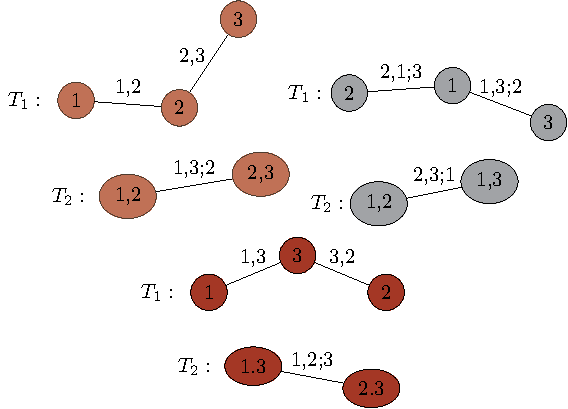
\includegraphics[width=0.8\linewidth]{03_PCC}
	
	\caption{Trzy możliwe dekompozycje 3-wymiarowego rozkładu przedstawione w postaci R-vine. \label{fig:PCCs}}
\end{figure}

Widzimy zatem, że Vine Copula są przydatnym narzędziem pozwalającym na tworzenie bardzo elastycznych modeli, mających na celu lepsze, bardziej skrojone na wymiar uchwycenie struktury zależności w danych.\\
W kolejnym rozdziale opiszemy finansowe \emph{spready} będące funkcją ceny kilku aktywów rynkowych. Zaprezentujemy kilka sposobów na ich modelowanie, i pokażemy bardzo generalną metodę wykorzystującą Vine Copulas.